\section{Результаты}
\label{sec:Results}

В данном разделе приводятся основные полученные в работе результаты, а также выполняется их детальный анализ.

\subsection{Название параграфа}
\label{sec:}

\begin{table*}[!h]
\caption{Пример простой таблицы, содержащей описательную статистику.}
\label{tab:tab_descr_1}
\setlength{\arrayrulewidth}{1.05 pt}
\renewcommand{\arraystretch}{1.1}
\begin{tabular*}{1.0\textwidth}{@{\extracolsep{\fill}}lrr}
\hline
Параметр & Название колонки & Название колонки \\
\hline
Среднее, $\mu$ & 0.79 & 0.98 \\
\hline
\end{tabular*}
\begin{spacing}{0.5}
{\scriptsize Пояснения: Здесь даются пояснения к таблице.}
\end{spacing}
\end{table*}

\subsection{Название параграфа}
\label{sec:}

\begin{table*}[!h]
\caption{Пример более сложной таблицы, содержащей оценки параметров модели.}
\label{tab:}
\setlength{\arrayrulewidth}{1.05 pt}
\renewcommand{\arraystretch}{1.1}
\begin{tabular*}{1.0\textwidth}{@{\extracolsep{\fill}}lrrr}
\hline
Параметр & \textit{Название колонки} & \textit{Название колонки} & \textit{Название колонки} \\
\hline

\multicolumn{4}{l}{\textit{Группа 1}} \\
$\mu$ & 0.30\textsuperscript{***} {\footnotesize (0.01)} & 0.30\textsuperscript{***} {\footnotesize (0.01)} & 0.30\textsuperscript{***} {\footnotesize (0.01)} \\
$\phi$ & 0.30\textsuperscript{***} {\footnotesize (0.01)} & 0.30\textsuperscript{***} {\footnotesize (0.01)} & 0.30\textsuperscript{***} {\footnotesize (0.01)} \\

\multicolumn{4}{l}{\textit{Группа 2}} \\
$\mu$ & 0.40\textsuperscript{*} {\footnotesize (0.17)} & 0.40\textsuperscript{*} {\footnotesize (0.17)} & 0.40\textsuperscript{*} {\footnotesize (0.17)} \\
$\phi$ & 0.40\textsuperscript{*} {\footnotesize (0.17)} & 0.40\textsuperscript{*} {\footnotesize (0.17)} & 0.40\textsuperscript{*} {\footnotesize (0.17)} \\

\hline
\end{tabular*}
\begin{spacing}{0.5}
{\scriptsize Пояснения: В скобках приведены стандартные ошибки параметров. Уровни значимости: *** -- 1\%, ** -- 5\%, * -- 10\%.}
\end{spacing}
\end{table*}

\subsection{Название параграфа}
\label{sec:}

\begin{figure*}[!h]
\centering
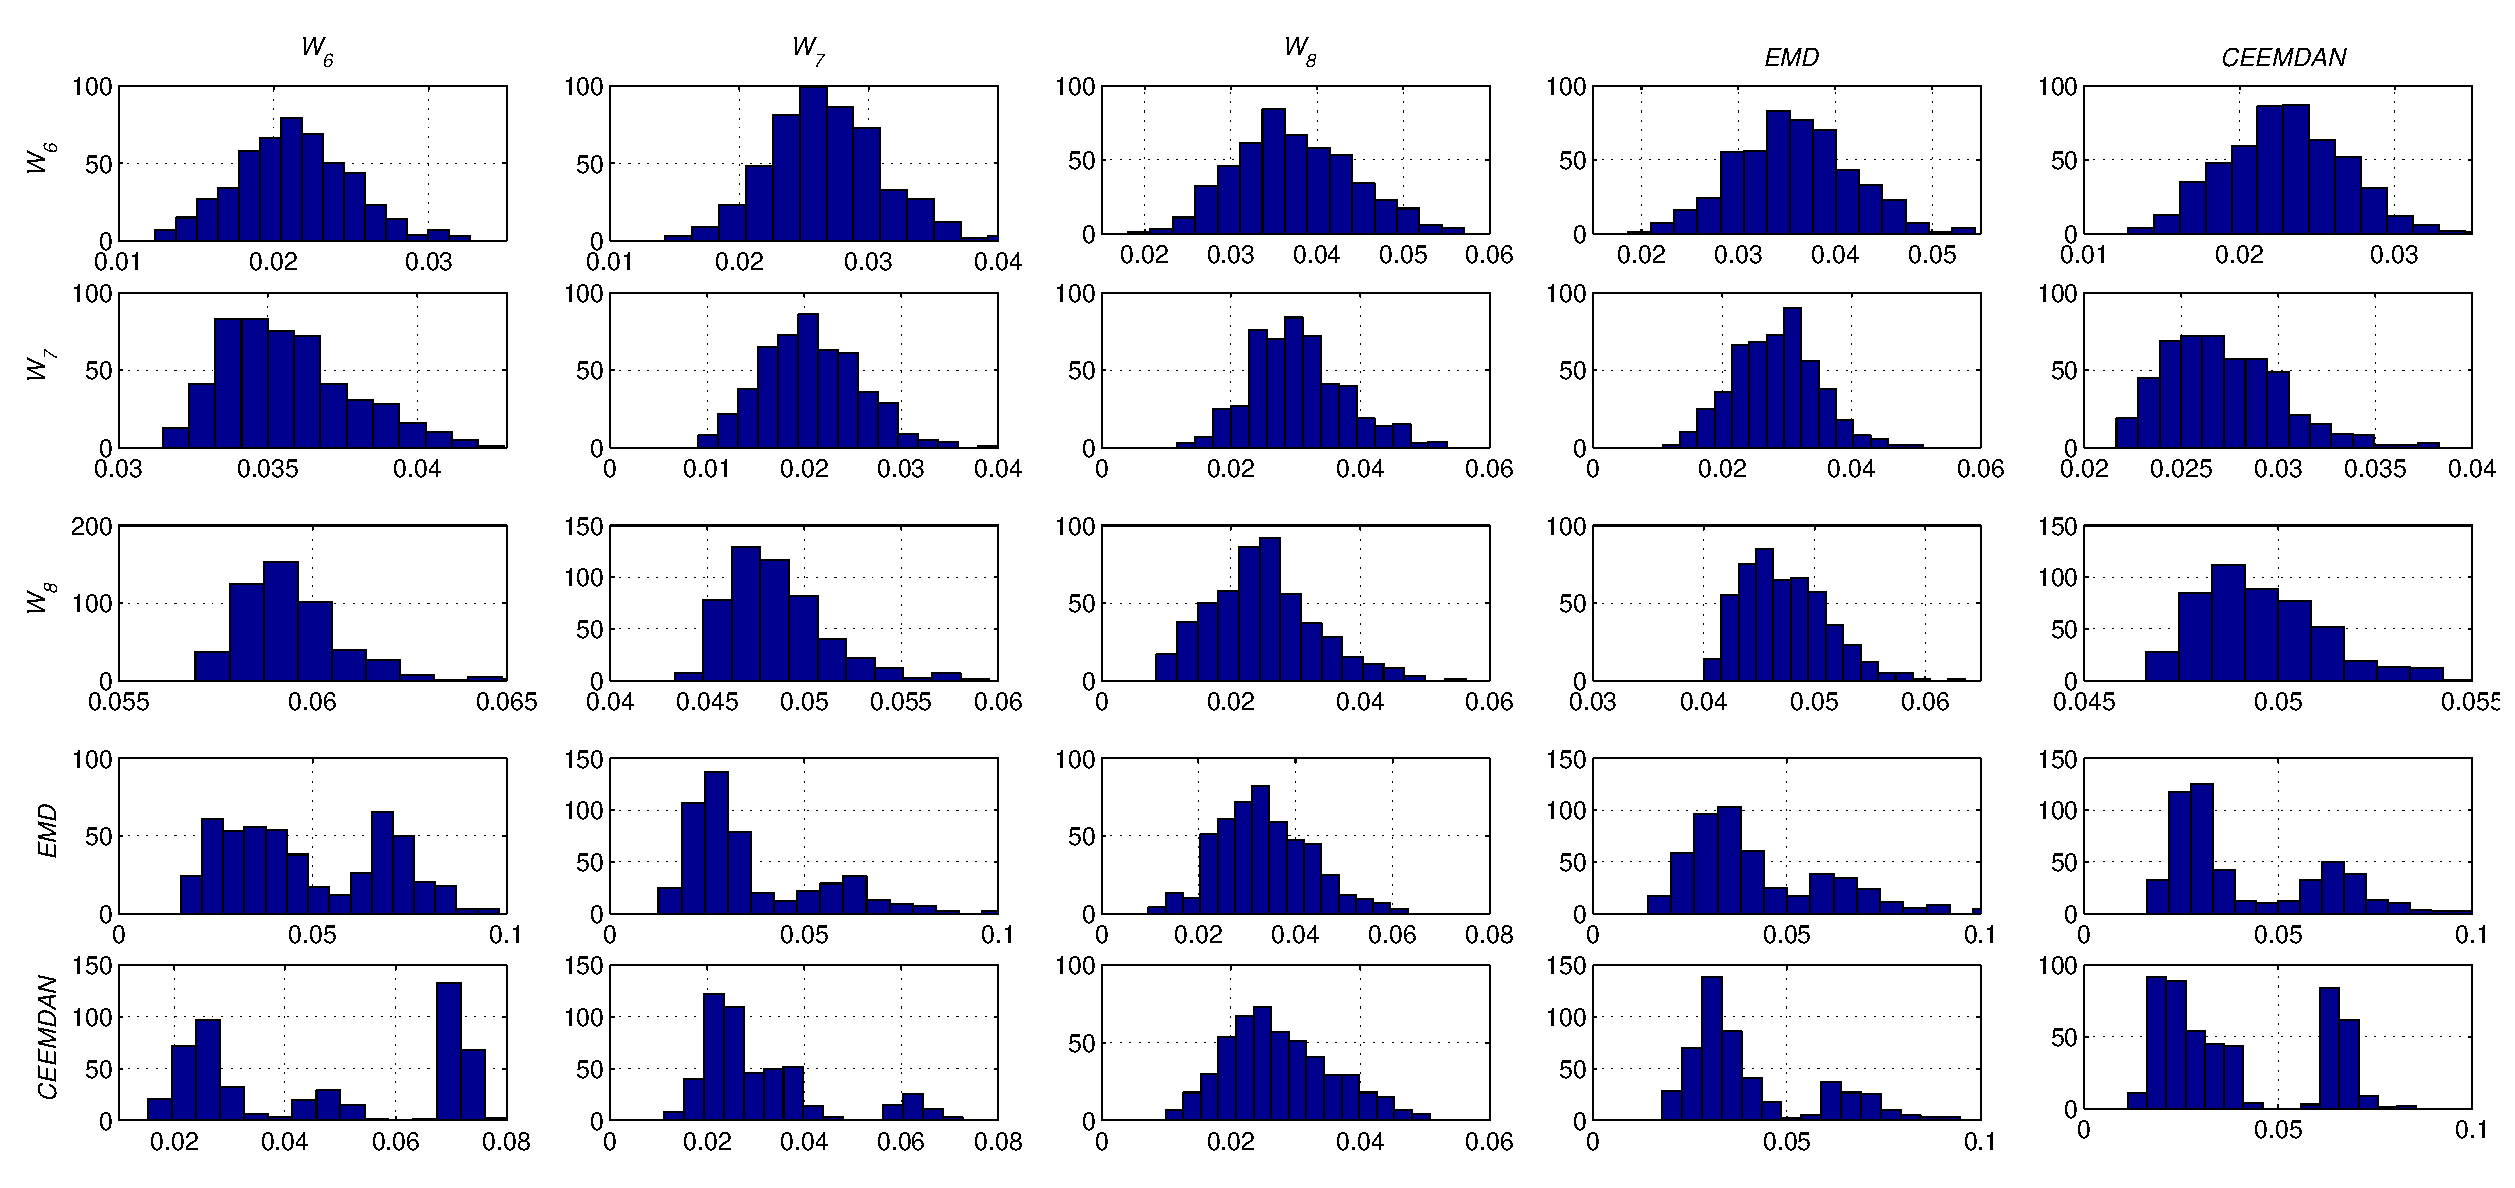
\includegraphics[width=1.0\textwidth,keepaspectratio]{Figure}
\caption{Название рисунка.}
\label{fig:}
\end{figure*}